\documentclass[11pt]{article}
\usepackage[letterpaper,margin=1in]{geometry}
\usepackage{amsmath,amssymb,bm,booktabs,graphicx,hyperref}
\hypersetup{hidelinks}
\setlength{\parindent}{0pt}
\setlength{\parskip}{0.35em}
\setlength{\emergencystretch}{2em}
\title{CS 577 Deep Learning\\Homework 3: Attention and Transformer Forward}
\author{Your Name (Hawk username: \texttt{yourname})}
\date{Fall 2026}
\begin{document}
\maketitle
\section*{Part 0: Setup and Axes}
All experiments were executed on a CPU with a fixed random seed of
\texttt{577}. The notebook environment used the following versions:

\begin{itemize}
    \item Python: \texttt{3.11.18}
    \item NumPy: \texttt{2.4.6}
    \item PyTorch: \texttt{2.15.0}
    \item Matplotlib: \texttt{3.11.2}
    \item Device: \texttt{CPU}
\end{itemize}

All 11 public tests passed successfully. These tests covered stable
masked softmax, causal masking, scaled dot-product attention,
head splitting and merging, multi-head self-attention and
cross-attention, positional encodings, and Transformer block behavior.

The final test summary was:

\begin{verbatim}
    Ran 11 tests in 0.047s

    OK

    Public-test return code: 0
\end{verbatim}

No failures or errors were reported.

\subsection*{0.2 Axis and mask contract}
% Define each axis, S/A/Y shapes, softmax axis, and (B,1,1,Tk) key mask.
The attention scores $S$, attention weights $A$, and output $Y$
have the following shapes:

\[
S: (B, H, T_q, T_k), \qquad
A: (B, H, T_q, T_k), \qquad
Y: (B, H, T_q, d_v).
\]

Here, $B$ is the batch size, $H$ is the number of heads,
$T_q$ is the number of query tokens, $T_k$ is the number
of key tokens, $d_k$ is the query/key feature size,
and $d_v$ is the value feature size.

We apply softmax along the last axis ($T_k$) because
each query compares itself with all keys. Softmax gives
a probability to each allowed key, and these probabilities
add up to 1. If all keys are blocked, the probabilities
are all zero.

The key mask first has shape $(B, T_k)$. We reshape it
to $(B, 1, 1, T_k)$ because each batch may have a different
mask, but the same mask is used for all heads and queries
within that batch.

NumPy broadcasting works by matching dimensions from
right to left. A dimension of size 1 can expand to match
the corresponding dimension in another array.

This allows the mask with shape $(B, 1, 1, T_k)$ to work
with attention scores of shape $(B, H, T_q, T_k)$.
\section*{Part 1: Hand Calculation}
The given query, key, and value matrices are:

\[
Q=K=
\begin{bmatrix}
1 & 0\\
0 & 1\\
1 & 1
\end{bmatrix},
\qquad
V=
\begin{bmatrix}
1 & 0\\
0 & 2\\
3 & 1
\end{bmatrix}.
\]

All three matrices have shape $(3,2)$, and $d_k=d_v=2$.

First, we calculate the dot products between queries
and keys:

\[
QK^\top=
\begin{bmatrix}
1 & 0 & 1\\
0 & 1 & 1\\
1 & 1 & 2
\end{bmatrix}.
\]

The shape of $QK^\top$ is $(3,3)$.

Next, we divide each score by $\sqrt{d_k}=\sqrt{2}$:

\[
S=\frac{QK^\top}{\sqrt{2}}
=
\begin{bmatrix}
0.7071 & 0 & 0.7071\\
0 & 0.7071 & 0.7071\\
0.7071 & 0.7071 & 1.4142
\end{bmatrix}.
\]

The scaled score matrix $S$ has shape $(3,3)$.

We apply softmax along each row to calculate the
attention weights:

\[
A=\operatorname{softmax}(S)
=
\begin{bmatrix}
0.4011 & 0.1978 & 0.4011\\
0.1978 & 0.4011 & 0.4011\\
0.2483 & 0.2483 & 0.5035
\end{bmatrix}.
\]

The attention weight matrix $A$ has shape $(3,3)$.
Each row sums to one.

\paragraph{Softmax calculation for cat.}

The scaled scores for the cat row are:

\[
s_{\mathrm{cat}}=
\left[
0,\frac{1}{\sqrt{2}},\frac{1}{\sqrt{2}}
\right].
\]

The softmax formula is:

\[
a_j=\frac{e^{s_j}}{\sum_k e^{s_k}}.
\]

The common denominator is:

\[
e^0+e^{1/\sqrt{2}}+e^{1/\sqrt{2}}.
\]

Using this denominator, the attention weights are:

\[
a_{\mathrm{The}}
=
\frac{e^0}
{e^0+2e^{1/\sqrt{2}}}
\approx 0.1978,
\]

\[
a_{\mathrm{cat}}
=
a_{\mathrm{sleeps}}
=
\frac{e^{1/\sqrt{2}}}
{e^0+2e^{1/\sqrt{2}}}
\approx 0.4011.
\]

The attention weights for cat are:

\[
a_{\mathrm{cat,row}}
=
[0.1978,\ 0.4011,\ 0.4011].
\]

\paragraph{Attention output.}

The attention output is calculated by multiplying
the attention weights by the value matrix:

\[
Y=AV=
\begin{bmatrix}
1.6044 & 0.7967\\
1.4011 & 1.2033\\
1.7587 & 1.0000
\end{bmatrix}.
\]

The output matrix $Y$ has shape $(3,2)$.

\paragraph{Weighted sum for cat.}

The value vectors are:

\[
V_{\mathrm{The}}=[1,0],\qquad
V_{\mathrm{cat}}=[0,2],\qquad
V_{\mathrm{sleeps}}=[3,1].
\]

We multiply each value vector by its attention
weight and add the results:

\[
Y_{\mathrm{cat}}
=
0.1978[1,0]
+
0.4011[0,2]
+
0.4011[3,1].
\]

Calculating each output component separately gives:

\[
Y_{\mathrm{cat}}
=
\left[
0.1978(1)+0.4011(0)+0.4011(3),
\right.
\]

\[
\left.
0.1978(0)+0.4011(2)+0.4011(1)
\right].
\]

The final output for cat is:

\[
\boxed{
Y_{\mathrm{cat}}=[1.4011,\ 1.2033]
}
\]

\subsection*{1.2 Causal attention}
% Show each query's visible keys, mask, weights and outputs.
% Explain last-row equality and output feature width.
In causal attention, each query can attend only to
the current token and previous tokens. Future tokens
are blocked.

In our example:
\begin{itemize}
    \item The can attend only to The.
    \item cat can attend to The and cat.
    \item sleeps can attend to all three tokens.
\end{itemize}

We use the causal mask $M$, where 1 means allowed
and 0 means blocked:

\[
M=
\begin{bmatrix}
1 & 0 & 0\\
1 & 1 & 0\\
1 & 1 & 1
\end{bmatrix}.
\]

The mask has shape $(3,3)$.

After applying the mask and softmax, the attention
weights are:

\[
A_{\mathrm{causal}}=
\begin{bmatrix}
1.0000 & 0 & 0\\
0.3302 & 0.6698 & 0\\
0.2483 & 0.2483 & 0.5035
\end{bmatrix}.
\]

The weight matrix has shape $(3,3)$. Blocked keys
have attention weights of exactly zero.

The new attention output is:

\[
Y_{\mathrm{causal}}=A_{\mathrm{causal}}V
=
\begin{bmatrix}
1.0000 & 0\\
0.3302 & 1.3395\\
1.7587 & 1.0000
\end{bmatrix}.
\]

The output matrix has shape $(3,2)$.

\paragraph{Weighted sum for cat.}

The cat query can attend only to The and cat.
The sleeps token is blocked.

The attention weights for cat are:

\[
a_{\mathrm{cat}}=[0.3302,\ 0.6698,\ 0].
\]

Using the value vectors, we calculate:

\[
Y_{\mathrm{cat}}
=
0.3302[1,0]
+
0.6698[0,2]
+
0[3,1].
\]

Calculating the two output components separately:

\[
\begin{aligned}
Y_{\mathrm{cat}}
&=
\bigl[
0.3302(1)+0.6698(0)+0(3),\\
&\qquad
0.3302(0)+0.6698(2)+0(1)
\bigr]\\
&\approx [0.3302,\ 1.3396].
\end{aligned}
\]

\textbf{Why the last row does not change:} The last token, sleeps, can attend to all three
tokens because there are no future tokens after it.
Therefore, its attention weights and output remain
the same as in unmasked attention.

\textbf{Why each output has two values:} Each value vector has two features $d_v=2$.
Attention calculates a weighted sum of these vectors.
The causal mask changes which tokens are used,
but it does not change the number of output features. That's why each output vector still has two values.
\subsection*{1.3 Scaling and stability}
% Show variance before/after scaling and row-max cancellation in softmax.
The dot product between a query and a key is:

\[
s=q^\top k=\sum_{r=0}^{d_k-1}q_rk_r.
\]

We assume that all coordinates are mutually independent,
have zero mean, and unit variance:

\[
E[q_r]=E[k_r]=0,
\qquad
\operatorname{Var}(q_r)=\operatorname{Var}(k_r)=1.
\]

Using the variance formula and the zero mean:

\[
\begin{aligned}
\operatorname{Var}(q_r)
&=E[q_r^2]-(E[q_r])^2=1,\\
E[q_r^2]&=1.
\end{aligned}
\]

Similarly, $E[k_r^2]=1$.

For each product, independence gives:

\[
E[q_rk_r]=E[q_r]E[k_r]=0.
\]

\[
E[q_r^2k_r^2]
=E[q_r^2]E[k_r^2]=1.
\]

Therefore,

\[
\begin{aligned}
\operatorname{Var}(q_rk_r)
&=E[(q_rk_r)^2]-(E[q_rk_r])^2\\
&=1-0^2\\
&=1.
\end{aligned}
\]

Since all coordinates are mutually independent,
each product uses a different independent pair.
Therefore, the variances of the products add:

\[
\begin{aligned}
\operatorname{Var}(s)
&=\operatorname{Var}
\left(\sum_{r=0}^{d_k-1}q_rk_r\right)\\
&=\sum_{r=0}^{d_k-1}\operatorname{Var}(q_rk_r)\\
&=\sum_{r=0}^{d_k-1}1\\
&=\boxed{d_k}.
\end{aligned}
\]

After scaling by $\sqrt{d_k}$:

\[
s_{\mathrm{scaled}}=\frac{s}{\sqrt{d_k}}.
\]

Using $\operatorname{Var}(cX)=c^2\operatorname{Var}(X)$:

\[
\begin{aligned}
\operatorname{Var}(s_{\mathrm{scaled}})
&=\operatorname{Var}\left(\frac{s}{\sqrt{d_k}}\right)\\
&=\frac{1}{d_k}\operatorname{Var}(s)\\
&=\frac{d_k}{d_k}\\
&=\boxed{1}.
\end{aligned}
\]

\textbf{Why scaling is important:} Without scaling, the standard deviation of the
attention scores is $\sqrt{d_k}$. As $d_k$ grows,
the scores can become more spread out.

For two softmax weights, their ratio is:

\[
\frac{a_i}{a_j}=e^{s_i-s_j}.
\]

This means the ratio grows exponentially when
the difference between scores increases.
As a result, the largest score can receive almost
all the attention weight, while the others receive
values close to zero.

Dividing by $\sqrt{d_k}$ keeps the score variance
controlled and reduces this problem.

\textbf{Numerical stability:} For numerical stability, we subtract the maximum
score from each row before applying softmax:

\[
m=\max_j s_j.
\]

The softmax formula becomes:

\[
\begin{aligned}
\operatorname{softmax}(s_i)
&=\frac{e^{s_i}}{\sum_j e^{s_j}}\\
&=\frac{e^{s_i-m}e^m}
{\sum_j e^{s_j-m}e^m}\\
&=\frac{e^{s_i-m}}{\sum_j e^{s_j-m}}.
\end{aligned}
\]

The common factor $e^m$ cancels, so subtracting
the maximum does not change the softmax result.

After subtraction, the largest shifted score is
zero, and its exponential is:

\[
e^0=1.
\]

All other shifted scores are less than or equal
to zero, so their exponentials are at most one.

For a row with at least one allowed key, the
denominator contains at least one term equal to
one. Therefore, it is at least one, which avoids
division by zero and denominator underflow.

For example, consider the scores:

\[
[1000,\ 999,\ -1000].
\]

Computing $e^{1000}$ directly can cause overflow.
After subtracting the maximum, we obtain:

\[
[0,\ -1,\ -2000].
\]

The exponentials are now:

\[
[1,\ e^{-1},\ e^{-2000}].
\]

This makes the calculation numerically stable
without changing the softmax probabilities.

A fully masked row is handled separately by
returning zeros, as required by the implementation.
\section*{Part 2: Stable Masked Attention}
\subsection*{2.1 Numerical stability and fully blocked rows}
% Report the extreme-score and empty-row checks; explain your guard.
TODO
\subsection*{2.2 Hand-case agreement}
% Report differences between full-precision hand/reference values and code.
TODO
\subsection*{2.3 Padding and causal masks}
% Show both combined masks, padded/future weights, and padding perturbation error.
TODO
\section*{Part 3: Multi-Head Attention}
\subsection*{3.1 Shape trace, attention maps, and outputs}
\begin{center}
\begin{tabular}{lll}
\toprule
Stage & Meaning & Shape \\
\midrule
$X$ & input features & TODO \\
$XW_Q,XW_K,XW_V$ & projected features & TODO \\
$Q,K,V$ & after splitting heads & TODO \\
$S,A$ & scores and weights per head & TODO \\
Head outputs & weighted values per head & TODO \\
Merged outputs & concatenated head features & TODO \\
$Y_{\mathrm{MHA}}$ & after output projection & TODO \\
\bottomrule
\end{tabular}
\end{center}
% Include the two maps and final output. Explain projection before splitting.
% Example: 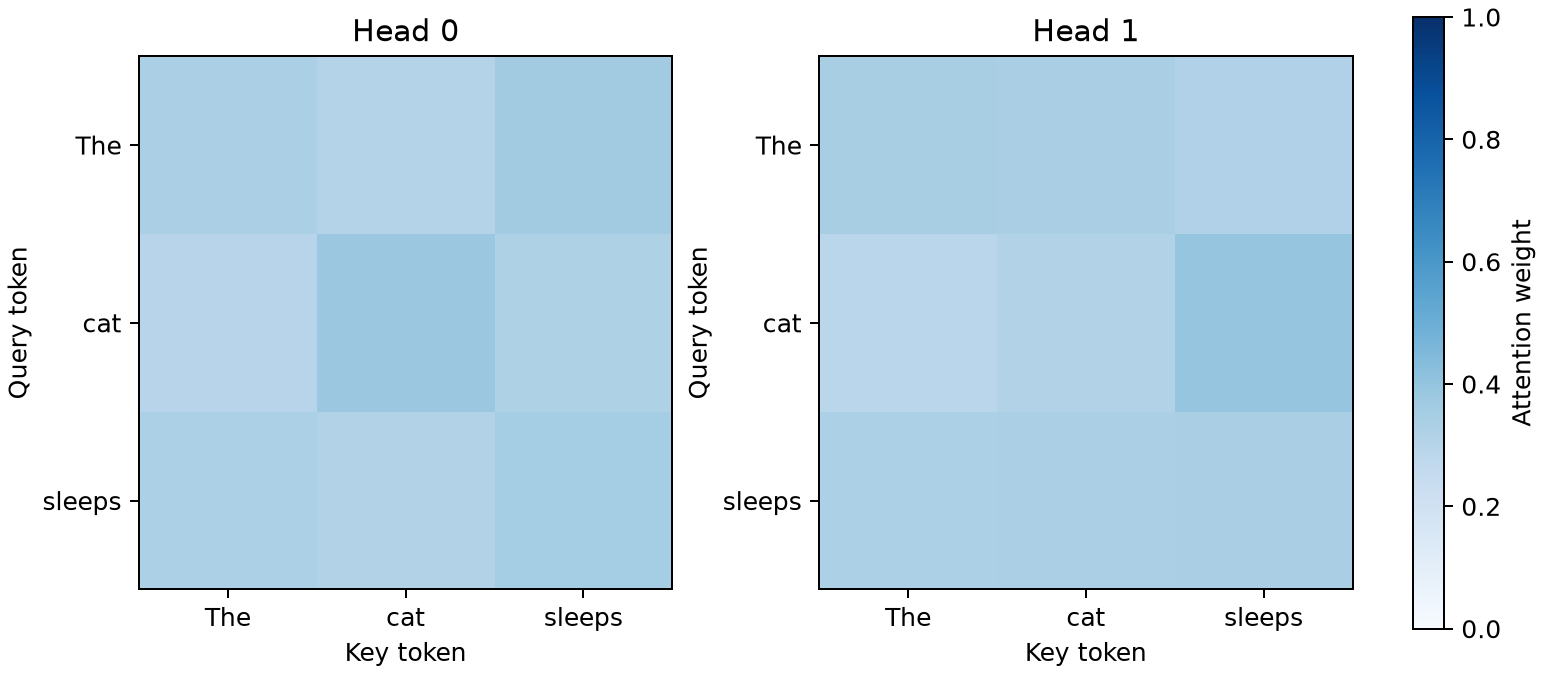
\includegraphics[width=.95\linewidth]{hw3_attention_maps.png}
TODO
\subsection*{3.2 Independent PyTorch comparison}
\begin{center}
\begin{tabular}{lrr}
\toprule
Case & Maximum output error & Maximum weight error \\
\midrule
Unmasked self-attention & TODO & TODO \\
Causal self-attention & TODO & TODO \\
Rectangular cross-attention & TODO & TODO \\
\bottomrule
\end{tabular}
\end{center}
% State parameter mapping and mask conventions.
TODO
\subsection*{3.3 Head count and head-output ablation}
% H=1 vs H=2: widths, scores, counts, output difference.
% Zero each head output before merging; report both changes and interpretation.
TODO
\section*{Part 4: Transformer Block}
\subsection*{4.1 Shape trace and reference checks}
% N1/U/N2/F/Z, independent PyTorch error and zero-update residual check.
TODO
\subsection*{4.2 Positions and reordering}
% All PE rows, feature-wise addition, two permutation errors and interpretation.
TODO
\subsection*{4.3 Future perturbation and causal visibility}
% First-two-position errors with and without masking; interpret each module.
TODO
\section*{Part 5: Architecture Comparison}
\subsection*{5.1 Encoder--decoder and decoder-only generation}
% Trace BOS->Le and Le->chat; identify queries and source K/V.
% Decoder-only prompt last position predicts Le; explain causal prefill.
TODO
\section*{Assistance and Generative-AI Disclosure}
% Name each tool/person, purpose, and what you independently verified/changed.
% If none, use the exact disclosure sentence in the assignment.
TODO
\end{document}
